\documentclass[task=1]{standalone}
\usepackage{setspace}
\usepackage{xcolor}
\usepackage[most]{tcolorbox}
% \usepackage{pgfplots}
% \pgfplotsset{compat=1.15}
% \pgfplotsset{soldot/.style={only marks,mark=*, line width=0.2pt, mark size=3pt, color=orange}}
% \pgfplotsset{holdot/.style={fill=white,only marks,mark=*, line width=1.0pt, mark size=1.5pt}}

\usepackage{tikz}
\usepackage{pgfplots}
\newcommand{\kariert}[3]{
  \footnotesize #1 \normalsize\newline
  \begin{tikzpicture}
    \draw[step=0.5cm, color=gray!50] (0,0) grid (#2 cm, #3 cm);
  \end{tikzpicture}
}

\begin{document}
 
 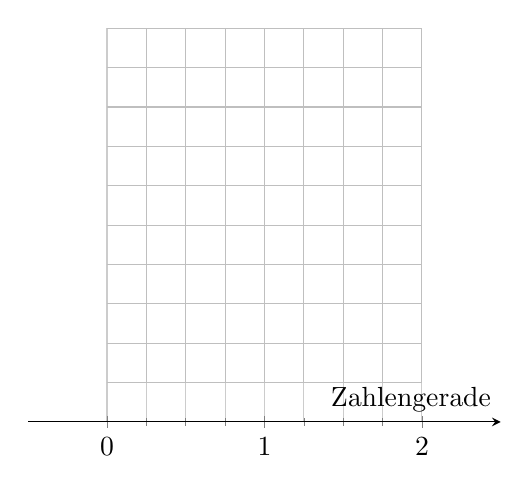
\begin{tikzpicture}
\begin{axis}[
    scale only axis,
    x=2cm,
    y=2cm,
    grid=both,
    minor tick num=3,
    grid style={solid, gray!40},
    axis lines=middle,
    axis y line=none,
    inner axis line style={=>},
    xlabel={Zahlengerade},
    ylabel={},
    yticklabel style={inner ysep=0pt, anchor=east, color=white},
    ytick={0,1,...,2},
    xticklabel style={inner xsep=0pt, anchor=north},
    xtick={0,1,...,2},
    ymin=0,
    ymax=2.5,
    xmin=-.5,
    xmax=2.5,
]
% \addplot[color=blue!70!red,thick,samples=100] {x^2};
% \node[] at (axis cs: 2.5,2) {$f(x) = x^2$};
\end{axis}
\draw[step=0.5cm, color=gray!50] (1,.5) grid (5 cm, 5 cm);
\end{tikzpicture}

\end{document}
% den Flächeninhalt 
% dem Graphen
% $x$-Achse
